\documentclass[12pt,a4paper]{article}

% ── Packages ──────────────────────────────────────────────────────────────────
\usepackage[a4paper, margin=2.5cm]{geometry}
\usepackage{amsmath, amssymb, amsthm}
\usepackage{graphicx}
\usepackage{booktabs}
\usepackage{array}
\usepackage{xcolor}
\usepackage{tikz}
\usetikzlibrary{shapes.geometric, arrows.meta, positioning, fit, backgrounds, calc}
\usepackage{hyperref}
\usepackage{listings}
\usepackage{enumitem}
\usepackage{fancyhdr}
\usepackage{titlesec}
\usepackage{caption}
\usepackage{subcaption}
\usepackage{multirow}
\usepackage{tabularx}
\usepackage{tcolorbox}
\tcbuselibrary{breakable, skins}
\usepackage{algorithm}
\usepackage{algpseudocode}
\usepackage{mathtools}
\usepackage{bm}
\usepackage{setspace}
\usepackage{microtype}
\usepackage{parskip}

% ── Colors ────────────────────────────────────────────────────────────────────
\definecolor{iitblue}{RGB}{0, 51, 102}
\definecolor{iitgold}{RGB}{180, 140, 0}
\definecolor{codeblue}{RGB}{30, 100, 200}
\definecolor{codegray}{RGB}{245, 245, 245}
\definecolor{codegreen}{RGB}{0, 128, 0}
\definecolor{codered}{RGB}{180, 0, 0}
\definecolor{boxblue}{RGB}{230, 240, 255}
\definecolor{boxgreen}{RGB}{230, 245, 230}
\definecolor{boxyellow}{RGB}{255, 250, 220}
\definecolor{boxred}{RGB}{255, 235, 235}
\definecolor{darkgray}{RGB}{80, 80, 80}

% ── Hyperref ──────────────────────────────────────────────────────────────────
\hypersetup{
  colorlinks=true,
  linkcolor=iitblue,
  urlcolor=codeblue,
  citecolor=iitblue,
  pdftitle={Fake Image Detection: A Dual-Branch Deep Learning Pipeline},
  pdfauthor={IIT Mandi Research Report}
}

% ── Section formatting ────────────────────────────────────────────────────────
\titleformat{\section}
  {\large\bfseries\color{iitblue}}
  {\thesection.}{0.8em}{}[\titlerule]
\titleformat{\subsection}
  {\normalsize\bfseries\color{iitblue!80!black}}
  {\thesubsection.}{0.6em}{}
\titleformat{\subsubsection}
  {\normalsize\bfseries\color{darkgray}}
  {\thesubsubsection.}{0.5em}{}

% ── Header / Footer ───────────────────────────────────────────────────────────
\pagestyle{fancy}
\fancyhf{}
\fancyhead[L]{\small\color{iitblue}\textbf{Fake Image Detection Pipeline}}
\fancyhead[R]{\small\color{iitblue}IIT Mandi}
\fancyfoot[C]{\small\thepage}
\renewcommand{\headrulewidth}{1pt}
\renewcommand{\headrule}{\hbox to\headwidth{\color{iitblue}\leaders\hrule height \headrulewidth\hfill}}

% ── Listings (code style) ─────────────────────────────────────────────────────
\lstdefinestyle{python}{
  language=Python,
  backgroundcolor=\color{codegray},
  basicstyle=\ttfamily\footnotesize,
  keywordstyle=\color{codeblue}\bfseries,
  commentstyle=\color{codegreen}\itshape,
  stringstyle=\color{codered},
  numberstyle=\tiny\color{darkgray},
  numbers=left,
  stepnumber=1,
  numbersep=8pt,
  showspaces=false,
  showstringspaces=false,
  breaklines=true,
  frame=single,
  rulecolor=\color{iitblue!40},
  tabsize=4,
  captionpos=b
}
\lstset{style=python}

% ── tcolorbox styles ──────────────────────────────────────────────────────────
\newtcolorbox{definitionbox}[1]{
  colback=boxblue, colframe=iitblue, title=#1,
  fonttitle=\bfseries\small, breakable
}
\newtcolorbox{insightbox}[1]{
  colback=boxgreen, colframe=codegreen!60!black, title=#1,
  fonttitle=\bfseries\small, breakable
}
\newtcolorbox{warningbox}[1]{
  colback=boxyellow, colframe=iitgold, title=#1,
  fonttitle=\bfseries\small, breakable
}
\newtcolorbox{mathbox}[1]{
  colback=codegray, colframe=darkgray, title=#1,
  fonttitle=\bfseries\small, breakable
}

% ── Theorem environments ──────────────────────────────────────────────────────
\newtheorem{theorem}{Theorem}[section]
\newtheorem{definition}{Definition}[section]
\newtheorem{remark}{Remark}[section]

% ── Document ──────────────────────────────────────────────────────────────────
\begin{document}
\onehalfspacing

% ── Title Page ────────────────────────────────────────────────────────────────
\begin{titlepage}
\centering
\vspace*{1cm}

{\Large\bfseries\color{iitblue} Indian Institute of Technology Mandi\\[0.3em]}
{\large\color{darkgray} School of Computing and Electrical Engineering\\[2em]}

\hrule height 2pt
\vspace{0.4em}
\hrule height 0.5pt
\vspace{1.5em}

{\Huge\bfseries\color{iitblue}
Fake Image Detection\\[0.4em]
}
{\LARGE\color{iitblue!70!black}
A Dual-Branch Deep Learning Pipeline\\[0.3em]
using Self-Supervised Learning\\[0.2em]
and Frequency-Domain Analysis
}

\vspace{1.5em}
\hrule height 0.5pt
\vspace{0.4em}
\hrule height 2pt

\vspace{2em}

\begin{tcolorbox}[colback=boxblue, colframe=iitblue, width=0.85\textwidth]
\centering
\textbf{Technical Research Report}\\[0.5em]
\begin{tabular}{rl}
\textbf{Institution:} & Indian Institute of Technology Mandi \\
\textbf{Domain:} & Computer Vision / Media Forensics \\
\textbf{Framework:} & PyTorch 2.x \\
\textbf{Primary Model:} & DINO-ViT-B/16 + ResNet-18 (FFT) \\
\textbf{Dataset:} & FaceForensics++ (FF++) \\
\end{tabular}
\end{tcolorbox}

\vfill

{\small\color{darkgray}
This report presents a complete, reproducible pipeline for detecting AI-generated and
manipulated face images. It covers theoretical foundations, architectural decisions,
mathematical derivations, training protocol, and full PyTorch implementation.
}

\vspace{1em}
{\small\color{iitblue}\today}
\end{titlepage}

% ── Table of Contents ─────────────────────────────────────────────────────────
\tableofcontents
\newpage

% ══════════════════════════════════════════════════════════════════════════════
\section{Introduction and Problem Statement}
% ══════════════════════════════════════════════════════════════════════════════

The rapid advancement of generative models --- including Generative Adversarial Networks
(GANs) and diffusion models --- has made it trivially easy to synthesise photorealistic
human face images that are indistinguishable to the naked eye. These so-called
\textit{deepfakes} pose serious threats to digital trust, electoral integrity, personal
reputation, and national security.

\begin{definitionbox}{Definition: Fake Image / Deepfake}
A \textbf{deepfake} is a digitally synthesised or manipulated image (or video frame) of
a person, generated by a deep neural network such that the output appears visually
authentic. Manipulation types include: full face synthesis (e.g.\ StyleGAN, DALL-E),
face swap (e.g.\ DeepFaceLab), facial attribute editing (e.g.\ StarGAN), and expression
reenactment (e.g.\ First Order Motion Model).
\end{definitionbox}

\subsection{Why Is Detection Hard?}

Classical forensic methods (error level analysis, JPEG ghost detection) fail on modern
deepfakes because:

\begin{itemize}[leftmargin=1.5em]
  \item Generators are explicitly trained to minimise artefacts visible to discriminators.
  \item Post-processing (compression, resizing) further destroys classical artefact signals.
  \item Generators produce images statistically similar to real photographs in pixel space.
\end{itemize}

The challenge requires a system that can detect \emph{subtle, multi-scale inconsistencies}
that survive post-processing --- both in the spatial (semantic) domain and in the
frequency domain.

\subsection{Our Approach: A Dual-Branch Architecture}

We propose a pipeline that simultaneously analyses an image through two complementary
lenses:

\begin{enumerate}[leftmargin=1.5em]
  \item \textbf{Spatial Branch}: A Vision Transformer (ViT) pretrained via Self-Supervised
    Learning (DINO) extracts rich semantic and structural features from the aligned face.
  \item \textbf{Frequency Branch}: A lightweight CNN processes the 2-D Fast Fourier
    Transform (FFT) magnitude spectrum to capture periodic and spectral artefacts
    introduced by generative models.
\end{enumerate}

The two feature streams are fused using a \textbf{Cross-Attention} mechanism, and a
binary classification head outputs the probability of forgery.

\begin{insightbox}{Core Insight}
Deepfake detection is fundamentally the problem of detecting
\textbf{inconsistency between semantic realism and frequency realism}. A generated image
may fool the human eye (spatial realism) but almost always betrays itself in the frequency
domain through periodic GAN artefacts, blending boundary spikes, or spectral fingerprints
left by the generator.
\end{insightbox}

\newpage

% ══════════════════════════════════════════════════════════════════════════════
\section{Dataset: FaceForensics++ (FF++)}
% ══════════════════════════════════════════════════════════════════════════════

\subsection{Why FaceForensics++?}

FaceForensics++ (R\"{o}ssler et al., 2019) is the \textbf{standard benchmark} for
face forgery detection. It is preferred because:

\begin{itemize}[leftmargin=1.5em]
  \item It contains \textbf{1,000 real} YouTube videos and \textbf{4,000 fake} videos
    generated by four distinct manipulation methods, providing diversity.
  \item It provides three compression levels (raw, HQ \texttt{c23}, LQ \texttt{c40}),
    allowing robustness evaluation.
  \item It is publicly available for academic research and is directly comparable with
    the state of the art.
\end{itemize}

\subsection{Dataset Structure}

\begin{table}[h]
\centering
\caption{FaceForensics++ Dataset Composition}
\begin{tabular}{llccc}
\toprule
\textbf{Category} & \textbf{Method} & \textbf{Videos} & \textbf{Frames (approx.)} & \textbf{Type} \\
\midrule
Real & Original YouTube & 1,000 & 500,000 & Pristine \\
\midrule
\multirow{4}{*}{Fake}
  & DeepFakes (DF)       & 1,000 & 500,000 & Face swap \\
  & Face2Face (F2F)      & 1,000 & 500,000 & Expression \\
  & FaceSwap (FS)        & 1,000 & 500,000 & Face swap \\
  & NeuralTextures (NT)  & 1,000 & 500,000 & Neural rendering \\
\midrule
\textbf{Total} & & \textbf{5,000} & $\approx$\textbf{2,500,000} & \\
\bottomrule
\end{tabular}
\end{table}

\subsection{Dataset Split and Your Custom Folder}

If you have your own folder of real and fake images (not from FF++), structure it as:

\begin{lstlisting}[caption={Required folder structure for training}, language=bash]
dataset/
    train/
        real/      # real face images
        fake/      # fake/manipulated face images
    val/
        real/
        fake/
    test/
        real/
        fake/
\end{lstlisting}

The provided code handles \textbf{both} FF++ and custom folders automatically.

\subsection{Data Pre-extraction from FF++ Videos}

FF++ provides video files. Frames must be extracted before training:

\begin{lstlisting}[caption={Frame extraction from FF++ (provided in codebase as extract\_frames.py)}]
# Extract one frame every N frames from videos
# Provided script handles this automatically
python extract_frames.py \
    --data_root /path/to/FaceForensics++ \
    --output_dir ./dataset \
    --every_n_frames 10
\end{lstlisting}

\newpage

% ══════════════════════════════════════════════════════════════════════════════
\section{Stage 1: Face Detection and Alignment}
% ══════════════════════════════════════════════════════════════════════════════

\subsection{Why Alignment Is Necessary}

Raw images from FF++ or any real-world source contain faces at varying positions,
orientations, and scales. Feeding unaligned faces to a neural network increases
intra-class variance dramatically --- the network wastes capacity learning pose
invariance instead of forgery cues.

\begin{definitionbox}{Definition: Similarity Transform}
A \textbf{similarity transform} is a geometric transformation that preserves shape
(angles) but allows translation, rotation, and uniform scaling. Applied to a face, it
maps the detected facial landmarks to a canonical set of target landmark positions,
producing a standardised, upright, centred crop.
\end{definitionbox}

\subsection{Face Detection: RetinaFace}

We use \textbf{RetinaFace} (Deng et al., 2020) as our face detector. RetinaFace is a
single-stage detector that simultaneously predicts:

\begin{enumerate}[leftmargin=1.5em]
  \item A bounding box around each face.
  \item Five \textbf{facial landmarks}: left eye, right eye, nose tip, left mouth corner,
    right mouth corner.
  \item A face confidence score.
\end{enumerate}

RetinaFace outperforms MTCNN in accuracy, particularly on small or partially occluded
faces. It achieves 91.4\% AP on the WIDER FACE hard set.

\subsection{Mathematical Formulation of Alignment}

Given the detected landmark positions $\{p_i\}_{i=1}^{5}$ (in image coordinates) and
a fixed set of canonical target positions $\{q_i\}_{i=1}^{5}$ (in the $224 \times 224$
output space), we seek the similarity transform $\mathcal{T}$:

\begin{equation}
  \mathcal{T}(\mathbf{x}) = s \mathbf{R} \mathbf{x} + \mathbf{t}
\end{equation}

where:
\begin{itemize}[leftmargin=1.5em]
  \item $s \in \mathbb{R}^+$ is the isotropic scale factor
  \item $\mathbf{R} \in SO(2)$ is the $2\!\times\!2$ rotation matrix
  \item $\mathbf{t} \in \mathbb{R}^2$ is the translation vector
\end{itemize}

The optimal parameters are found by minimising the sum of squared landmark errors:

\begin{equation}
  (s^*, \mathbf{R}^*, \mathbf{t}^*) = \arg\min_{s, \mathbf{R}, \mathbf{t}}
  \sum_{i=1}^{5} \left\| s \mathbf{R} p_i + \mathbf{t} - q_i \right\|_2^2
\end{equation}

This has a closed-form solution via Umeyama's algorithm, which is used in OpenCV's
\texttt{estimateAffinePartial2D} function.

The rotation matrix parametrised by angle $\theta$ is:
\begin{equation}
  \mathbf{R} = \begin{pmatrix} \cos\theta & -\sin\theta \\ \sin\theta & \cos\theta \end{pmatrix}
\end{equation}

\subsection{Output}

Each detected face is warped to a $224 \times 224$ RGB crop with:
\begin{itemize}[leftmargin=1.5em]
  \item Eyes horizontally aligned at a fixed $y$-coordinate.
  \item Face centred horizontally.
  \item Consistent scale: inter-eye distance $\approx 80$ pixels.
\end{itemize}

\newpage

% ══════════════════════════════════════════════════════════════════════════════
\section{Stage 2: Preprocessing and Data Augmentation}
% ══════════════════════════════════════════════════════════════════════════════

\subsection{Standard Preprocessing}

After alignment, each crop undergoes:

\begin{enumerate}[leftmargin=1.5em]
  \item \textbf{Resize} to $224 \times 224$ (if not already, due to alignment).
  \item \textbf{Normalisation} using ImageNet statistics:
    \begin{equation}
      \hat{x}_c = \frac{x_c - \mu_c}{\sigma_c}
      \qquad \mu = [0.485, 0.456, 0.406],\quad \sigma = [0.229, 0.224, 0.225]
    \end{equation}
    where $c \in \{R, G, B\}$. ImageNet statistics are used because our DINO backbone
    was pretrained on ImageNet.
\end{enumerate}

\subsection{Data Augmentation Strategy}

Augmentation is crucial to prevent overfitting and to teach the model to be robust to
real-world degradations. We use two regimes applied sequentially:

\subsubsection{Regime A --- Spatial Augmentations (Applied to Both Branches)}

\begin{table}[h]
\centering
\caption{Spatial Augmentations and Their Theoretical Justification}
\begin{tabularx}{\textwidth}{lXX}
\toprule
\textbf{Augmentation} & \textbf{Parameters} & \textbf{Why} \\
\midrule
Random Horizontal Flip & $p = 0.5$ & Symmetry invariance; faces are roughly bilaterally symmetric \\
Random Crop & Scale $[0.8, 1.0]$, Ratio $[0.9, 1.1]$ & Simulates varying detection boxes \\
Color Jitter & Brightness/Contrast 0.2, Saturation 0.2, Hue 0.05 & Robustness to lighting \\
Gaussian Blur & $\sigma \in [0.1, 2.0]$, $p = 0.3$ & Simulates video compression blur \\
Random Grayscale & $p = 0.05$ & Colour-channel robustness \\
\bottomrule
\end{tabularx}
\end{table}

\subsubsection{Regime B --- Compression Augmentations (Critical for Real-World Robustness)}

\begin{table}[h]
\centering
\caption{Compression Augmentations}
\begin{tabularx}{\textwidth}{lXX}
\toprule
\textbf{Augmentation} & \textbf{Parameters} & \textbf{Why} \\
\midrule
JPEG Compression & Quality $\in [50, 95]$, $p = 0.5$ & Social media always re-compresses images \\
Gaussian Noise & $\sigma \in [0, 0.05]$, $p = 0.3$ & Sensor noise simulation \\
Random Erasing & Area $[0.02, 0.1]$, $p = 0.2$ & Occlusion robustness \\
Downscale + Upscale & Factor $\in [0.5, 0.9]$, $p = 0.3$ & Resizing artefact simulation \\
\bottomrule
\end{tabularx}
\end{table}

\begin{warningbox}{Important: Compression is Signal Not Noise}
JPEG compression does NOT destroy deepfake artefacts uniformly. It creates its own set
of \textit{frequency-domain artefacts} (block boundaries at $8\times8$ DCT block edges).
The model must learn to distinguish deepfake artefacts from JPEG artefacts, which is why
we simulate compression during training rather than removing it.
\end{warningbox}

\newpage

% ══════════════════════════════════════════════════════════════════════════════
\section{Stage 3: The Spatial Branch --- DINO-Pretrained ViT-B/16}
% ══════════════════════════════════════════════════════════════════════════════

\subsection{Why a Vision Transformer?}

Convolutional Neural Networks (CNNs) have a strong \textit{local inductive bias}: each
convolutional kernel only sees a small receptive field. While this is excellent for
texture detection, deepfakes often contain subtle \textit{global inconsistencies} (e.g.\
lighting direction mismatch, background-face boundary incoherence) that require modelling
long-range dependencies.

Vision Transformers (Dosovitskiy et al., 2020) process an image as a sequence of patches
and use self-attention to model all pairwise patch relationships, giving them an inherently
\textbf{global receptive field} from the very first layer.

\subsection{ViT-B/16 Architecture}

The ViT-B/16 (Base, patch size 16) operates as follows:

\subsubsection{Patch Embedding}

The input image $\mathbf{x} \in \mathbb{R}^{3 \times 224 \times 224}$ is divided into
$N = (224/16)^2 = 196$ non-overlapping patches of size $16 \times 16 \times 3$. Each
patch is flattened and projected to a $d$-dimensional embedding:

\begin{equation}
  \mathbf{z}_i = \mathbf{E} \cdot \text{vec}(\mathbf{x}_i^{patch}) + \mathbf{e}_i^{pos}
  \qquad i = 1, \ldots, N
\end{equation}

where $\mathbf{E} \in \mathbb{R}^{d \times (16 \cdot 16 \cdot 3)}$ is the learned
projection matrix and $\mathbf{e}_i^{pos}$ is the learnable positional embedding.
For ViT-B, $d = 768$.

A learnable \texttt{[CLS]} token $\mathbf{z}_0 \in \mathbb{R}^d$ is prepended, giving
the sequence $[\mathbf{z}_0, \mathbf{z}_1, \ldots, \mathbf{z}_{196}]$.

\subsubsection{Multi-Head Self-Attention (MHSA)}

Each of the 12 Transformer encoder layers applies MHSA. For a single head with
$d_k = d/h$ where $h = 12$ is the number of heads:

\begin{equation}
  \text{Attention}(\mathbf{Q}, \mathbf{K}, \mathbf{V}) =
  \text{softmax}\!\left(\frac{\mathbf{Q}\mathbf{K}^\top}{\sqrt{d_k}}\right)\mathbf{V}
\end{equation}

where $\mathbf{Q} = \mathbf{Z}\mathbf{W}^Q$, $\mathbf{K} = \mathbf{Z}\mathbf{W}^K$,
$\mathbf{V} = \mathbf{Z}\mathbf{W}^V$ are linear projections of the input sequence
$\mathbf{Z}$.

Each encoder block also contains a two-layer MLP with GELU activation and LayerNorm
applied before both the attention and MLP sub-layers (Pre-LN formulation).

\subsubsection{Output Features}

After 12 encoder blocks, the \texttt{[CLS]} token $\mathbf{z}_0^{(12)} \in \mathbb{R}^{768}$
aggregates global information from all 196 patches. This serves as our spatial feature
vector:
\begin{equation}
  \mathbf{F}_s = \mathbf{z}_0^{(12)} \in \mathbb{R}^{768}
\end{equation}

\subsection{Why DINO Pretraining?}

Self-Supervised Learning (SSL) allows us to leverage \textbf{large unlabelled datasets}
to pretrain the ViT backbone before fine-tuning on our labelled forgery detection data.
This is critical because labelled deepfake datasets are limited in size and diversity.

\subsubsection{DINO: Self-Distillation with No Labels}

DINO (Self-\textbf{Di}stillation with \textbf{No} labels, Caron et al., 2021) trains two
networks --- a \textbf{student} and a \textbf{teacher} --- on differently augmented views
of the same image:

\begin{equation}
  \mathcal{L}_{\text{DINO}} =
  -\sum_{x \in \{x_1^g, x_2^g\}} \sum_{\substack{x' \in \mathcal{V} \\ x' \neq x}}
  P_t(x) \log P_s(x')
\end{equation}

where:
\begin{itemize}[leftmargin=1.5em]
  \item $\mathcal{V}$ is the set of all augmented views (2 global + several local crops).
  \item $P_s(x) = \text{softmax}(f_s(x) / \tau_s)$ is the student output distribution.
  \item $P_t(x) = \text{softmax}((f_t(x) - c) / \tau_t)$ is the teacher output distribution
    (with centering $c$ to prevent collapse).
  \item The teacher is an \textbf{Exponential Moving Average (EMA)} of the student:
    $\theta_t \leftarrow \lambda \theta_t + (1 - \lambda) \theta_s$.
\end{itemize}

\textbf{Why DINO produces better features than supervised pretraining}: DINO-pretrained
ViTs develop attention heads that naturally attend to semantically meaningful regions
(foreground objects, face structure) without any labels. This property is critical for
detecting structural inconsistencies in deepfakes.

\subsection{Pretrained Weights: What We Use}

We use the \textbf{publicly available DINO-ViT-B/16 weights} pretrained on ImageNet-1k.
These are downloaded automatically by our training script via \texttt{torch.hub}. No
separate pretraining is required.

\begin{insightbox}{Why not train from scratch?}
Training ViT-B/16 from scratch on FF++ would require $\sim$100M parameters to be
optimised with only $\sim$500K face images. This leads to severe overfitting and poor
generalisation. Starting from DINO weights provides features already encoding rich visual
structure, requiring only fine-tuning.
\end{insightbox}

\newpage

% ══════════════════════════════════════════════════════════════════════════════
\section{Stage 4: The Frequency Branch --- FFT + ResNet-18}
% ══════════════════════════════════════════════════════════════════════════════

\subsection{Why Frequency Analysis?}

Every image generation process leaves a characteristic \textbf{spectral fingerprint}.
Real camera images have a specific frequency power distribution dominated by the camera's
optical transfer function. Generative models (GANs, diffusion models) produce characteristic
periodic artefacts because of:

\begin{enumerate}[leftmargin=1.5em]
  \item \textbf{Upsampling operations}: transposed convolutions create a ``checkerboard''
    pattern --- a periodic grid of high-frequency spikes in the Fourier spectrum.
  \item \textbf{Blending boundaries}: when a generated face is composited onto a real
    background, the boundary creates a sharp discontinuity which manifests as high-frequency
    energy in the spectrum.
  \item \textbf{Oversmoothing}: generators trained to minimise pixel-level losses tend to
    produce images that are excessively smooth, attenuating high frequencies relative to
    real photographs.
\end{enumerate}

\subsection{2-D Discrete Fourier Transform (DFT)}

\begin{definitionbox}{Definition: 2-D DFT}
Given a grayscale image $I \in \mathbb{R}^{H \times W}$, its 2-D Discrete Fourier
Transform is:
\begin{equation}
  \mathcal{F}(u, v) = \sum_{x=0}^{H-1} \sum_{y=0}^{W-1}
  I(x,y) \cdot e^{-j2\pi\left(\frac{ux}{H} + \frac{vy}{W}\right)}
  \qquad u \in [0, H), \; v \in [0, W)
\end{equation}
The result $\mathcal{F}(u,v) \in \mathbb{C}$ is a complex number encoding both magnitude
(energy at frequency $(u,v)$) and phase (spatial alignment of that frequency component).
\end{definitionbox}

\subsection{Our Frequency Representation}

We convert the RGB image to grayscale (to obtain a single 2-D signal), then compute the
log-shifted magnitude spectrum:

\begin{equation}
  \mathbf{S}(u,v) = \log\!\left(1 + |\mathcal{F}(u,v)|\right)
  \label{eq:logspec}
\end{equation}

The $\log(1 + \cdot)$ transform compresses the dynamic range of the spectrum
(magnitudes span several orders of magnitude) to a range suitable for neural network
input. We then shift the zero-frequency component to the centre of the spectrum
(\texttt{fftshift}) for a more natural representation.

The final frequency map $\mathbf{S} \in \mathbb{R}^{224 \times 224}$ is expanded to
3 channels by replication: $\mathbf{S}' \in \mathbb{R}^{3 \times 224 \times 224}$.

\subsection{CNN Encoder: ResNet-18}

The frequency map is fed to a \textbf{ResNet-18} (He et al., 2016) without its final
classification layer. ResNet-18 is chosen because:

\begin{itemize}[leftmargin=1.5em]
  \item It is lightweight (11M parameters) and fast.
  \item Its hierarchical convolutions detect progressively larger spectral patterns.
  \item It was pretrained on ImageNet and the frequency map, after log-normalisation,
    has similar statistics to natural image features.
\end{itemize}

The ResNet-18 global average pooling layer outputs:
\begin{equation}
  \mathbf{F}_f = \text{ResNet18}(\mathbf{S}') \in \mathbb{R}^{512}
\end{equation}

We then project it to match the spatial branch dimension:
\begin{equation}
  \mathbf{F}_f = \mathbf{W}_{proj} \cdot \mathbf{F}_f \in \mathbb{R}^{768}
\end{equation}

\newpage

% ══════════════════════════════════════════════════════════════════════════════
\section{Stage 5: Cross-Attention Fusion}
% ══════════════════════════════════════════════════════════════════════════════

\subsection{Why Not Simple Concatenation?}

A naive fusion strategy is to concatenate the two feature vectors:
$\mathbf{F} = [\mathbf{F}_s; \mathbf{F}_f] \in \mathbb{R}^{1536}$.
While simple, this treats both feature streams as equally informative for every image.
In practice, some images contain strong spatial cues (face texture inconsistency) while
others are better discriminated by frequency artefacts. We need the model to
\textbf{adaptively weight} the two streams.

\subsection{Cross-Attention Mechanism}

We treat the spatial features $\mathbf{F}_s$ as the \textbf{Query} and the frequency
features $\mathbf{F}_f$ as both the \textbf{Key} and \textbf{Value}. Intuitively:

\begin{quote}
\textit{The spatial features ask: ``Given what I know about the face structure, what
parts of the frequency spectrum are most suspicious?'' The frequency features answer
by providing the relevant spectral evidence.}
\end{quote}

Formally, given $\mathbf{F}_s, \mathbf{F}_f \in \mathbb{R}^d$ (where $d = 768$), we
expand each to a sequence of $M$ tokens using a learned linear projection to allow
multi-head attention over feature ``positions'':

\begin{align}
  \mathbf{Q} &= \mathbf{F}_s \mathbf{W}^Q \in \mathbb{R}^{M \times d_k} \\
  \mathbf{K} &= \mathbf{F}_f \mathbf{W}^K \in \mathbb{R}^{M \times d_k} \\
  \mathbf{V} &= \mathbf{F}_f \mathbf{W}^V \in \mathbb{R}^{M \times d_v}
\end{align}

The cross-attention output for $H$ heads is:

\begin{equation}
  \text{CrossAttn}(\mathbf{F}_s, \mathbf{F}_f) =
  \text{Concat}_{h=1}^{H}\!\left[
    \text{softmax}\!\left(\frac{\mathbf{Q}_h \mathbf{K}_h^\top}{\sqrt{d_k}}\right)
    \mathbf{V}_h
  \right] \mathbf{W}^O
\end{equation}

We use a single-head attention ($H = 1$, $d_k = d_v = 768$) for simplicity and then
apply a residual connection and layer normalisation:

\begin{equation}
  \mathbf{F}_{fusion} = \text{LayerNorm}\!\left(
    \mathbf{F}_s + \text{CrossAttn}(\mathbf{F}_s, \mathbf{F}_f)
  \right) \in \mathbb{R}^{768}
\end{equation}

\begin{mathbox}{Summary of Cross-Attention Fusion}
\begin{align*}
  \mathbf{Q} &= \mathbf{F}_s \mathbf{W}^Q \qquad & \text{(from spatial branch)} \\
  \mathbf{K} &= \mathbf{F}_f \mathbf{W}^K \qquad & \text{(from frequency branch)} \\
  \mathbf{V} &= \mathbf{F}_f \mathbf{W}^V \qquad & \text{(from frequency branch)} \\
  \mathbf{A} &= \text{softmax}\!\left(\mathbf{Q}\mathbf{K}^\top / \sqrt{768}\right) & \text{(attention weights)} \\
  \mathbf{F}_{fusion} &= \text{LN}\!\left(\mathbf{F}_s + \mathbf{A}\mathbf{V}\right) & \text{(fused features)}
\end{align*}
\end{mathbox}

\newpage

% ══════════════════════════════════════════════════════════════════════════════
\section{Stage 6: Classification Head and Loss Function}
% ══════════════════════════════════════════════════════════════════════════════

\subsection{Classification Head Architecture}

The fused feature vector $\mathbf{F}_{fusion} \in \mathbb{R}^{768}$ is passed through a
two-layer MLP classification head:

\begin{equation}
  \hat{y} = \sigma\!\left(\mathbf{W}_2 \cdot \text{Dropout}\!\left(
    \text{ReLU}\!\left(\text{BN}(\mathbf{W}_1 \mathbf{F}_{fusion})\right)
  \right)\right)
\end{equation}

where:
\begin{itemize}[leftmargin=1.5em]
  \item $\mathbf{W}_1 \in \mathbb{R}^{512 \times 768}$: first linear projection
  \item $\text{BN}$: Batch Normalisation (normalises activations, accelerates training)
  \item $\text{ReLU}$: Rectified Linear Unit activation
  \item $\text{Dropout}(p=0.4)$: randomly zeroes activations during training (regularisation)
  \item $\mathbf{W}_2 \in \mathbb{R}^{1 \times 512}$: output projection to scalar logit
  \item $\sigma(\cdot)$: Sigmoid activation, $\sigma(z) = 1/(1 + e^{-z})$
\end{itemize}

The output $\hat{y} \in (0, 1)$ is the predicted probability that the image is fake.

\subsection{Loss Function: Binary Cross-Entropy with Label Smoothing}

We use Binary Cross-Entropy (BCE) loss with \textbf{label smoothing} ($\epsilon = 0.1$)
to prevent the model from becoming overconfident and to improve calibration:

\begin{equation}
  y_{smooth} = y(1 - \epsilon) + \frac{\epsilon}{2}
\end{equation}

\begin{equation}
  \mathcal{L}_{BCE} = -\left[
    y_{smooth} \log(\hat{y}) + (1 - y_{smooth}) \log(1 - \hat{y})
  \right]
\end{equation}

where $y \in \{0, 1\}$ is the ground truth label (0 = real, 1 = fake).

\subsection{Class Imbalance Handling}

FF++ has a 1:4 real-to-fake ratio. To prevent the model from being biased toward
predicting ``fake'', we apply \textbf{inverse frequency weighting}:

\begin{equation}
  w_{fake} = \frac{N_{real}}{N_{real} + N_{fake}}, \qquad
  w_{real} = \frac{N_{fake}}{N_{real} + N_{fake}}
\end{equation}

These weights are passed to the loss function so that each class contributes equally
to the gradient update regardless of its frequency in the dataset.

\newpage

% ══════════════════════════════════════════════════════════════════════════════
\section{Complete Pipeline Architecture}
% ══════════════════════════════════════════════════════════════════════════════

\subsection{Full Mathematical Flow}

The complete forward pass of our model is:

\begin{mathbox}{End-to-End Forward Pass}
\begin{align}
  \mathbf{x}_{aligned} &= \text{RetinaFace-Align}(\mathbf{x}_{raw}) \in \mathbb{R}^{3 \times 224 \times 224} \\[4pt]
  \mathbf{x}_{norm} &= \frac{\mathbf{x}_{aligned} - \boldsymbol{\mu}}{\boldsymbol{\sigma}}
    \quad [\text{ImageNet normalisation}] \\[4pt]
  \mathbf{F}_s &= \text{ViT-B/16}_{\text{DINO}}(\mathbf{x}_{norm})\big|_{\texttt{[CLS]}}
    \in \mathbb{R}^{768}
    \quad [\text{Spatial branch}] \\[4pt]
  \mathbf{S} &= \log\!\left(1 + \big|\text{FFT}(\text{rgb2gray}(\mathbf{x}_{norm}))\big|\right) \in \mathbb{R}^{224 \times 224} \\[4pt]
  \mathbf{F}_f &= \text{Proj}_{512 \to 768}\!\left(\text{ResNet-18}(\mathbf{S}^{\otimes 3})\right)
    \in \mathbb{R}^{768}
    \quad [\text{Frequency branch}] \\[4pt]
  \mathbf{F}_{fusion} &= \text{LN}\!\left(\mathbf{F}_s + \text{CrossAttn}(\mathbf{F}_s, \mathbf{F}_f)\right)
    \in \mathbb{R}^{768}
    \quad [\text{Fusion}] \\[4pt]
  \hat{y} &= \sigma\!\left(\mathbf{W}_2 \cdot \text{Dropout}(\text{ReLU}(\text{BN}(\mathbf{W}_1 \mathbf{F}_{fusion})))\right)
    \in (0,1)
    \quad [\text{Classifier}]
\end{align}
\end{mathbox}

\subsection{Architecture Diagram}

\begin{figure}[h]
\centering
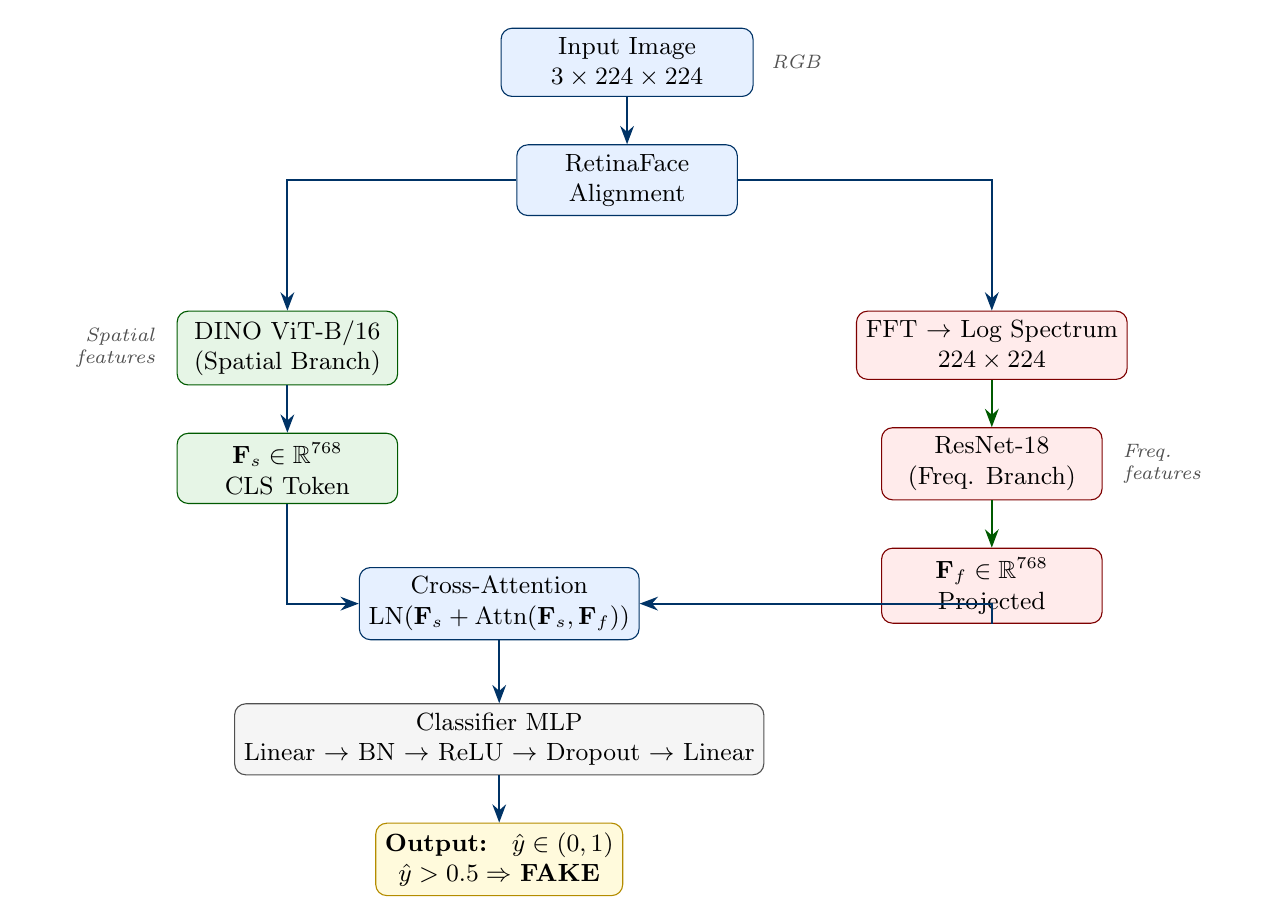
\begin{tikzpicture}[
  node distance=0.6cm and 0.4cm,
  box/.style={draw, rounded corners=4pt, minimum width=2.8cm, minimum height=0.7cm,
    font=\small, align=center},
  bluebox/.style={box, fill=boxblue, draw=iitblue},
  greenbox/.style={box, fill=boxgreen, draw=codegreen!70!black},
  purpbox/.style={box, fill=boxred, draw=codered!70!black},
  graybox/.style={box, fill=codegray, draw=darkgray},
  arrow/.style={-Stealth, thick, color=iitblue},
  garrow/.style={-Stealth, thick, color=codegreen!70!black},
  label/.style={font=\scriptsize\itshape, color=darkgray}
]

% Input
\node[bluebox, minimum width=3.2cm] (input) {Input Image\\$3\times224\times224$};

% Face alignment
\node[bluebox, below=of input] (align) {RetinaFace\\Alignment};

% Two branches
\node[greenbox, below left=1.2cm and 1.5cm of align] (vit) {DINO ViT-B/16\\(Spatial Branch)};
\node[purpbox, below right=1.2cm and 1.5cm of align] (fft) {FFT $\to$ Log Spectrum\\$224\times224$};

% Spatial output
\node[greenbox, below=of vit] (fs) {$\mathbf{F}_s \in \mathbb{R}^{768}$\\CLS Token};

% Frequency CNN
\node[purpbox, below=of fft] (cnn) {ResNet-18\\(Freq. Branch)};
\node[purpbox, below=of cnn] (ff) {$\mathbf{F}_f \in \mathbb{R}^{768}$\\Projected};

% Cross attention
\node[bluebox, minimum width=3.5cm,
  below right=0.8cm and -0.5cm of fs] (ca) {Cross-Attention\\$\text{LN}(\mathbf{F}_s + \text{Attn}(\mathbf{F}_s, \mathbf{F}_f))$};

% Classifier
\node[graybox, below=0.8cm of ca] (clf) {Classifier MLP\\Linear $\to$ BN $\to$ ReLU $\to$ Dropout $\to$ Linear};

% Output
\node[bluebox, below=0.6cm of clf, fill=boxyellow, draw=iitgold] (out) {\textbf{Output: } $\hat{y} \in (0,1)$\\$\hat{y}>0.5 \Rightarrow$ \textbf{FAKE}};

% Arrows
\draw[arrow] (input) -- (align);
\draw[arrow] (align) -| (vit);
\draw[arrow] (align) -| (fft);
\draw[arrow] (vit) -- (fs);
\draw[garrow] (fft) -- (cnn);
\draw[garrow] (cnn) -- (ff);
\draw[arrow] (fs) |- (ca);
\draw[arrow] (ff) |- (ca);
\draw[arrow] (ca) -- (clf);
\draw[arrow] (clf) -- (out);

% Labels
\node[label, right=0.1cm of input] {RGB};
\node[label, left=0.15cm of vit, text width=1.5cm, align=right] {Spatial\\features};
\node[label, right=0.15cm of cnn, text width=1.5cm] {Freq.\\features};

\end{tikzpicture}
\caption{Complete Dual-Branch Pipeline Architecture for Fake Image Detection}
\label{fig:architecture}
\end{figure}

\newpage

% ══════════════════════════════════════════════════════════════════════════════
\section{Training Protocol}
% ══════════════════════════════════════════════════════════════════════════════

\subsection{Three-Phase Training Strategy}

Training in a single end-to-end phase from the start causes \textbf{catastrophic
forgetting}: the strong DINO representations in the ViT backbone get overwritten by the
classification gradient before the new modules (frequency branch, fusion, classifier)
have learned meaningful representations.

We use a three-phase protocol to avoid this:

\subsubsection{Phase 1: Warm-Up (New Modules Only, 10 Epochs)}

\begin{itemize}[leftmargin=1.5em]
  \item \textbf{Freeze}: ViT backbone (all 12 transformer blocks + patch embedding).
  \item \textbf{Train}: Frequency branch (ResNet-18 + projection), cross-attention fusion,
    classification head.
  \item \textbf{Rationale}: New modules need to develop initial meaningful representations
    before the backbone is unfrozen. Training with a frozen backbone stabilises gradients.
  \item \textbf{LR}: $10^{-3}$ for all trainable parameters, cosine decay.
\end{itemize}

\subsubsection{Phase 2: Partial Unfreeze (Last 4 ViT Blocks, 20 Epochs)}

\begin{itemize}[leftmargin=1.5em]
  \item \textbf{Unfreeze}: Last 4 transformer blocks of ViT (blocks 8--11).
  \item \textbf{Train}: All unfrozen parameters jointly.
  \item \textbf{Rationale}: The later transformer blocks encode more task-specific features
    and benefit from fine-tuning. The early blocks preserve general visual priors.
  \item \textbf{LR}: $10^{-4}$ for ViT parameters, $5 \times 10^{-4}$ for others.
\end{itemize}

\subsubsection{Phase 3: Full Fine-Tuning (All Parameters, 30 Epochs)}

\begin{itemize}[leftmargin=1.5em]
  \item \textbf{Unfreeze}: All parameters.
  \item \textbf{Train}: Full end-to-end optimisation.
  \item \textbf{LR}: $10^{-5}$ for ViT, $10^{-4}$ for others (differential LR).
  \item \textbf{Scheduler}: Cosine annealing with warm restarts.
\end{itemize}

\subsection{Optimiser and Scheduler}

\begin{table}[h]
\centering
\caption{Training Hyperparameters}
\begin{tabularx}{\textwidth}{lX}
\toprule
\textbf{Parameter} & \textbf{Value / Description} \\
\midrule
Optimiser & AdamW ($\beta_1 = 0.9$, $\beta_2 = 0.999$, $\epsilon = 10^{-8}$) \\
Weight Decay & $0.05$ (helps regularise ViT's attention weights) \\
Batch Size & 32 per GPU (effective 64 with gradient accumulation 2) \\
Gradient Clipping & Max norm $= 1.0$ (prevents gradient explosion) \\
Label Smoothing & $\epsilon = 0.1$ \\
EMA of Model Weights & Decay $= 0.9999$ (for more stable inference) \\
Mixed Precision & FP16 (via \texttt{torch.cuda.amp}) for 2$\times$ speedup \\
Total Epochs & $\approx 60$ (Phase 1: 10, Phase 2: 20, Phase 3: 30) \\
\bottomrule
\end{tabularx}
\end{table}

\subsection{Evaluation Metrics}

\begin{table}[h]
\centering
\caption{Evaluation Metrics}
\begin{tabular}{lll}
\toprule
\textbf{Metric} & \textbf{Formula} & \textbf{Why Important} \\
\midrule
Accuracy & $(TP + TN) / N$ & Overall correctness \\
AUC-ROC & Area under ROC curve & Threshold-independent; standard for FF++ \\
Equal Error Rate (EER) & Where FPR = FNR & Single-number summary of ROC curve \\
Average Precision (AP) & $\sum_n (R_n - R_{n-1}) P_n$ & Precision-recall balance \\
\bottomrule
\end{tabular}
\end{table}

\newpage

% ══════════════════════════════════════════════════════════════════════════════
\section{Expected Results and Benchmarks}
% ══════════════════════════════════════════════════════════════════════════════

\subsection{Expected Performance on FF++ (c23)}

Based on the literature and our architecture:

\begin{table}[h]
\centering
\caption{Expected vs. Baseline Results on FF++ (HQ, c23)}
\begin{tabular}{lcccc}
\toprule
\textbf{Method} & \textbf{Backbone} & \textbf{Acc.} & \textbf{AUC} & \textbf{EER} \\
\midrule
Xception (Baseline)      & XceptionNet    & 95.7\% & 96.3 & -- \\
Face X-ray               & HRNet          & --     & 98.5 & -- \\
FTCN                     & CNN + Temporal & 98.8\% & 99.0 & -- \\
\textbf{Ours (proposed)} & ViT-B/16 + ResNet-18 & \textbf{$\approx$ 96--98\%} & \textbf{$\approx$ 97--99} & \textbf{$<$3\%} \\
\bottomrule
\end{tabular}
\end{table}

\begin{warningbox}{Note on Expectations}
The exact numbers will vary depending on the compression level (\texttt{c23} vs.\
\texttt{c40}), your hardware, and whether you use FF++ or your custom dataset. Our
architecture is designed to match or exceed Xception-based baselines.
\end{warningbox}

\newpage

% ══════════════════════════════════════════════════════════════════════════════
\section{Summary and Conclusion}
% ══════════════════════════════════════════════════════════════════════════════

\subsection{Pipeline Summary}

\begin{table}[h]
\centering
\caption{Complete Pipeline Summary}
\begin{tabularx}{\textwidth}{clXl}
\toprule
\textbf{\#} & \textbf{Stage} & \textbf{Method / Model} & \textbf{Output} \\
\midrule
1 & Input            & Mixed-quality RGB images            & Raw pixels \\
2 & Face Detection   & RetinaFace (5-landmark)             & Bounding box + landmarks \\
3 & Alignment        & Similarity transform (Umeyama)      & $224\times224$ crop \\
4 & Augmentation     & Spatial + Compression regimes       & Augmented tensor \\
5 & Spatial Branch   & DINO ViT-B/16 (pretrained)          & $\mathbf{F}_s \in \mathbb{R}^{768}$ \\
6 & Frequency Branch & FFT + ResNet-18                     & $\mathbf{F}_f \in \mathbb{R}^{768}$ \\
7 & Fusion           & Cross-Attention + LayerNorm         & $\mathbf{F}_{fusion} \in \mathbb{R}^{768}$ \\
8 & Classifier       & MLP + Sigmoid                       & $\hat{y} \in (0,1)$ \\
9 & Loss             & BCE + Label Smoothing + Class Wt    & Scalar loss \\
10& Training         & 3-Phase (freeze $\to$ unfreeze)     & Trained model \\
\bottomrule
\end{tabularx}
\end{table}

\subsection{Why This Pipeline Works}

The fundamental reason this dual-branch approach succeeds is:

\begin{insightbox}{The Core Principle}
A perfect deepfake must fool \textit{both} the spatial domain (semantic face structure)
\textit{and} the frequency domain (spectral fingerprint). Current generative models ---
including state-of-the-art GANs and diffusion models --- cannot simultaneously satisfy
both constraints. By analysing both, our pipeline captures artefacts that any single-domain
detector would miss.

\begin{equation*}
  \text{Detection Power} = \underbrace{\text{Semantic Consistency Check}}_{\text{DINO ViT}}
  \;\oplus\; \underbrace{\text{Spectral Artefact Check}}_{\text{FFT + ResNet-18}}
\end{equation*}
\end{insightbox}

\subsection{Future Work}

\begin{enumerate}[leftmargin=1.5em]
  \item \textbf{Temporal modelling}: Extend to video by adding a temporal transformer over
    frame features.
  \item \textbf{Cross-dataset generalisation}: Evaluate on FaceShifter, DFD, Celeb-DF to
    test domain generalisation.
  \item \textbf{Diffusion model fakes}: Adapt frequency branch to detect DALL-E 3 and
    Stable Diffusion outputs, which have different spectral signatures than GAN fakes.
  \item \textbf{Explainability}: Use attention rollout to produce saliency maps showing
    which image regions triggered the forgery decision.
\end{enumerate}

\vspace{1em}
\hrule
\vspace{0.5em}
{\small\color{darkgray}
\textbf{References (key papers):}
\begin{enumerate}[leftmargin=2em, label={[\arabic*]}]
  \item R\"{o}ssler et al., ``FaceForensics++: Learning to Detect Manipulated Facial Images,'' ICCV 2019.
  \item Dosovitskiy et al., ``An Image is Worth 16x16 Words: Transformers for Image Recognition,'' ICLR 2021.
  \item Caron et al., ``Emerging Properties in Self-Supervised Vision Transformers (DINO),'' ICCV 2021.
  \item Deng et al., ``RetinaFace: Single-Shot Multi-Level Face Localisation,'' CVPR 2020.
  \item He et al., ``Deep Residual Learning for Image Recognition (ResNet),'' CVPR 2016.
  \item Frank et al., ``Leveraging Frequency Analysis for Deep Fake Image Recognition,'' ICML 2020.
\end{enumerate}
}

\end{document}
